\section{Denoising}
\begin{frame}{}
    \LARGE Diffusion Models: \textbf{Denoising}
\end{frame}

\begin{frame}[allowframebreaks]{Denoising Diffusion Probabilistic Models}
    
Denoising diffusion models, also known as score-based generative models, have recently emerged as a powerful class of generative models. They achieve remarkable results in high-fidelity image generation, often outperforming GANs.
\begin{figure}
    \centering
    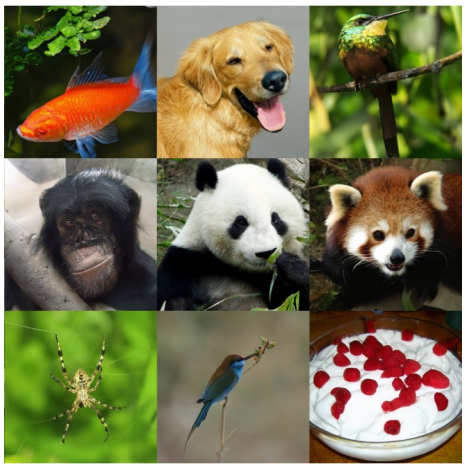
\includegraphics[height=0.5\textheight, width=\textwidth, keepaspectratio]{images/diffusion/diff_results_1.png}
    \caption*{Diffusion Models Beat GANs on Image Synthesis \href{https://arxiv.org/abs/2105.05233}{Dhariwal \& Nichol, OpenAI, 2021}}
\end{figure}

\framebreak
Denoising diffusion models consist of two processes:
\begin{itemize}
    \item A fixed (predefined) \textbf{forward diffusion process} $q$, which gradually adds Gaussian noise to an image until only pure noise remains.
    \item A learned \textbf{reverse denoising diffusion process} $p_\theta$, where a neural network is trained to gradually denoise an image starting from pure noise, eventually recovering the original image.
\end{itemize}

\begin{figure}
    \centering
    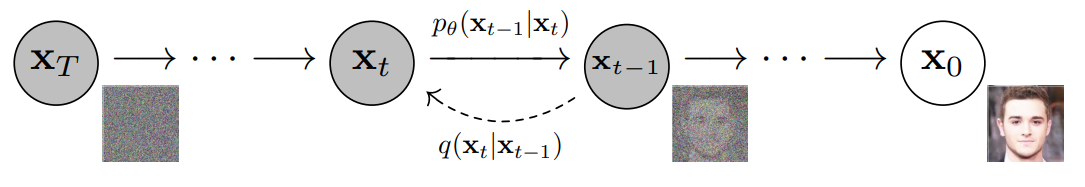
\includegraphics[height=0.8\textheight, width=\textwidth, keepaspectratio]{images/diffusion/diff_3.png}
\end{figure}

\framebreak

\begin{figure}
    \centering
    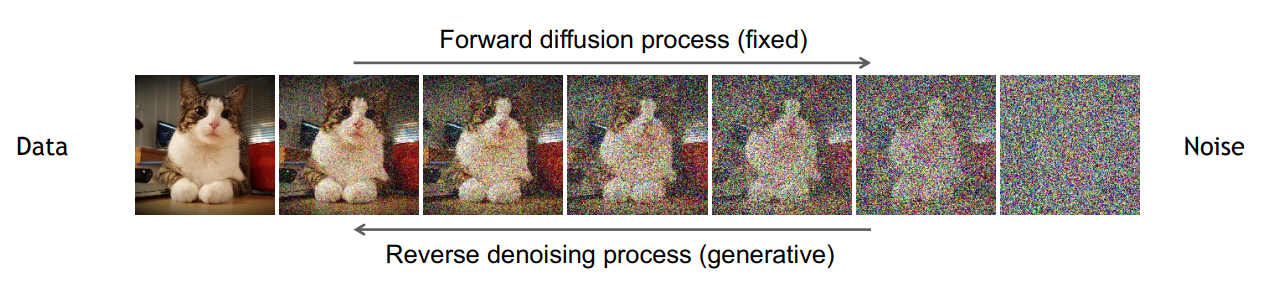
\includegraphics[height=0.9\textheight, width=\textwidth, keepaspectratio]{images/diffusion/diffusion_1.png}
\end{figure}

\end{frame}